% Options for packages loaded elsewhere
% Options for packages loaded elsewhere
\PassOptionsToPackage{unicode}{hyperref}
\PassOptionsToPackage{hyphens}{url}
%
\documentclass[
  english,
  russian,
  12pt,
  a4paper,
  DIV=11,
  numbers=noendperiod]{scrreprt}
\usepackage{xcolor}
\usepackage{amsmath,amssymb}
\setcounter{secnumdepth}{5}
\usepackage{iftex}
\ifPDFTeX
  \usepackage[T1]{fontenc}
  \usepackage[utf8]{inputenc}
  \usepackage{textcomp} % provide euro and other symbols
\else % if luatex or xetex
  \usepackage{unicode-math} % this also loads fontspec
  \defaultfontfeatures{Scale=MatchLowercase}
  \defaultfontfeatures[\rmfamily]{Ligatures=TeX,Scale=1}
\fi
\usepackage{lmodern}
\ifPDFTeX\else
  % xetex/luatex font selection
\fi
% Use upquote if available, for straight quotes in verbatim environments
\IfFileExists{upquote.sty}{\usepackage{upquote}}{}
\IfFileExists{microtype.sty}{% use microtype if available
  \usepackage[]{microtype}
  \UseMicrotypeSet[protrusion]{basicmath} % disable protrusion for tt fonts
}{}
\usepackage{setspace}
% Make \paragraph and \subparagraph free-standing
\makeatletter
\ifx\paragraph\undefined\else
  \let\oldparagraph\paragraph
  \renewcommand{\paragraph}{
    \@ifstar
      \xxxParagraphStar
      \xxxParagraphNoStar
  }
  \newcommand{\xxxParagraphStar}[1]{\oldparagraph*{#1}\mbox{}}
  \newcommand{\xxxParagraphNoStar}[1]{\oldparagraph{#1}\mbox{}}
\fi
\ifx\subparagraph\undefined\else
  \let\oldsubparagraph\subparagraph
  \renewcommand{\subparagraph}{
    \@ifstar
      \xxxSubParagraphStar
      \xxxSubParagraphNoStar
  }
  \newcommand{\xxxSubParagraphStar}[1]{\oldsubparagraph*{#1}\mbox{}}
  \newcommand{\xxxSubParagraphNoStar}[1]{\oldsubparagraph{#1}\mbox{}}
\fi
\makeatother


\usepackage{longtable,booktabs,array}
\usepackage{calc} % for calculating minipage widths
% Correct order of tables after \paragraph or \subparagraph
\usepackage{etoolbox}
\makeatletter
\patchcmd\longtable{\par}{\if@noskipsec\mbox{}\fi\par}{}{}
\makeatother
% Allow footnotes in longtable head/foot
\IfFileExists{footnotehyper.sty}{\usepackage{footnotehyper}}{\usepackage{footnote}}
\makesavenoteenv{longtable}
\usepackage{graphicx}
\makeatletter
\newsavebox\pandoc@box
\newcommand*\pandocbounded[1]{% scales image to fit in text height/width
  \sbox\pandoc@box{#1}%
  \Gscale@div\@tempa{\textheight}{\dimexpr\ht\pandoc@box+\dp\pandoc@box\relax}%
  \Gscale@div\@tempb{\linewidth}{\wd\pandoc@box}%
  \ifdim\@tempb\p@<\@tempa\p@\let\@tempa\@tempb\fi% select the smaller of both
  \ifdim\@tempa\p@<\p@\scalebox{\@tempa}{\usebox\pandoc@box}%
  \else\usebox{\pandoc@box}%
  \fi%
}
% Set default figure placement to htbp
\def\fps@figure{htbp}
\makeatother



\ifLuaTeX
\usepackage[bidi=basic,provide=*]{babel}
\else
\usepackage[bidi=default,provide=*]{babel}
\fi
% get rid of language-specific shorthands (see #6817):
\let\LanguageShortHands\languageshorthands
\def\languageshorthands#1{}


\setlength{\emergencystretch}{3em} % prevent overfull lines

\providecommand{\tightlist}{%
  \setlength{\itemsep}{0pt}\setlength{\parskip}{0pt}}



 
\usepackage[style=gost-numeric,backend=biber,langhook=extras,autolang=other*]{biblatex}
\addbibresource{bib/cite.bib}

\usepackage[]{csquotes}

\KOMAoption{captions}{tableheading}
\usepackage{indentfirst}
\usepackage{float}
\floatplacement{figure}{H}
\usepackage[math,RM={Scale=0.94},SS={Scale=0.94},SScon={Scale=0.94},TT={Scale=MatchLowercase,FakeStretch=0.9},DefaultFeatures={Ligatures=Common}]{plex-otf}
\makeatletter
\@ifpackageloaded{caption}{}{\usepackage{caption}}
\AtBeginDocument{%
\ifdefined\contentsname
  \renewcommand*\contentsname{Содержание}
\else
  \newcommand\contentsname{Содержание}
\fi
\ifdefined\listfigurename
  \renewcommand*\listfigurename{Список иллюстраций}
\else
  \newcommand\listfigurename{Список иллюстраций}
\fi
\ifdefined\listtablename
  \renewcommand*\listtablename{Список таблиц}
\else
  \newcommand\listtablename{Список таблиц}
\fi
\ifdefined\figurename
  \renewcommand*\figurename{Рисунок}
\else
  \newcommand\figurename{Рисунок}
\fi
\ifdefined\tablename
  \renewcommand*\tablename{Таблица}
\else
  \newcommand\tablename{Таблица}
\fi
}
\@ifpackageloaded{float}{}{\usepackage{float}}
\floatstyle{ruled}
\@ifundefined{c@chapter}{\newfloat{codelisting}{h}{lop}}{\newfloat{codelisting}{h}{lop}[chapter]}
\floatname{codelisting}{Список}
\newcommand*\listoflistings{\listof{codelisting}{Листинги}}
\makeatother
\makeatletter
\makeatother
\makeatletter
\@ifpackageloaded{caption}{}{\usepackage{caption}}
\@ifpackageloaded{subcaption}{}{\usepackage{subcaption}}
\makeatother
\usepackage{bookmark}
\IfFileExists{xurl.sty}{\usepackage{xurl}}{} % add URL line breaks if available
\urlstyle{same}
\hypersetup{
  pdftitle={Отчет по лабораторной работе №3},
  pdfauthor={Мишина Анастасия Алексеевна},
  pdflang={ru-RU},
  hidelinks,
  pdfcreator={LaTeX via pandoc}}


\title{Отчет по лабораторной работе №3}
\usepackage{etoolbox}
\makeatletter
\providecommand{\subtitle}[1]{% add subtitle to \maketitle
  \apptocmd{\@title}{\par {\large #1 \par}}{}{}
}
\makeatother
\subtitle{Дисциплина: Моделирование сетей передачи данных}
\author{Мишина Анастасия Алексеевна}
\date{}
\begin{document}
\maketitle

\renewcommand*\contentsname{Содержание}
{
\setcounter{tocdepth}{1}
\tableofcontents
}
\listoffigures
\listoftables

\setstretch{1.5}
\chapter{Цель
работы}\label{ux446ux435ux43bux44c-ux440ux430ux431ux43eux442ux44b}

Основной целью работы является знакомство с инструментом для измерения
пропускной способности сети в режиме реального времени --- iPerf3, а
также получение навыков проведения воспроизводимого эксперимента по
измерению пропускной способности моделируемой сети в среде Mininet.

\chapter{Задание}\label{ux437ux430ux434ux430ux43dux438ux435}

\begin{enumerate}
\def\labelenumi{\arabic{enumi}.}
\tightlist
\item
  Воспроизвести посредством API Mininet эксперименты по измерению
  пропускной способности с помощью iPerf3.
\item
  Построить графики по проведённому эксперименту.
\end{enumerate}

\chapter{Теоретическое
введение}\label{ux442ux435ux43eux440ux435ux442ux438ux447ux435ux441ux43aux43eux435-ux432ux432ux435ux434ux435ux43dux438ux435}

Mininet\autocite{mininet} -- это эмулятор компьютерной сети. Под
компьютерной сетью подразумеваются простые компьютеры --- хосты,
коммутаторы, а так же OpenFlow-контроллеры. С помощью простейшего
синтаксиса в примитивном интерпретаторе команд можно разворачивать сети
из произвольного количества хостов, коммутаторов в различных топологиях
и все это в рамках одной виртуальной машины(ВМ). На всех хостах можно
изменять сетевую конфигурацию, пользоваться стандартными
утилитами(ifconfig, ping) и даже получать доступ к терминалу. На
коммутаторы можно добавлять различные правила и маршрутизировать трафик.

iPerf3\autocite{iperf} представляет собой кроссплатформенное
клиент-серверное приложение с открытым исходным кодом, которое можно
использовать для измерения пропускной способности между двумя конечными
устройствами. iPerf3 может работать с транспортными протоколами TCP, UDP
и SCTP:

\begin{itemize}
\tightlist
\item
  TCP и SCTP:

  \begin{itemize}
  \tightlist
  \item
    измеряет пропускную способность;
  \item
    позволяет задать размер MSS/MTU;
  \item
    отслеживает размер окна перегрузки TCP (CWnd).
  \end{itemize}
\item
  UDP:

  \begin{itemize}
  \tightlist
  \item
    измеряет пропускную способность;
  \item
    измеряет потери пакетов;
  \item
    измеряет колебания задержки (jitter);
  \item
    поддерживает групповую рассылку пакетов (multicast).
  \end{itemize}
\end{itemize}

\chapter{Выполнение лабораторной
работы}\label{ux432ux44bux43fux43eux43bux43dux435ux43dux438ux435-ux43bux430ux431ux43eux440ux430ux442ux43eux440ux43dux43eux439-ux440ux430ux431ux43eux442ux44b}

\section{Установка необходимого программного
обеспечения}\label{ux443ux441ux442ux430ux43dux43eux432ux43aux430-ux43dux435ux43eux431ux445ux43eux434ux438ux43cux43eux433ux43e-ux43fux440ux43eux433ux440ux430ux43cux43cux43dux43eux433ux43e-ux43eux431ux435ux441ux43fux435ux447ux435ux43dux438ux44f}

С помощью API Mininet создадим простейшую топологию сети, состоящую из
двух хостов и коммутатора с назначенной по умолчанию mininet сетью
10.0.0.0/8.

В каталоге /work/lab\_iperf3 для работы над проектом создадим подкаталог
lab\_iperf3\_topo и скопируем в него файл с примером скрипта
mininet/examples/emptynet.py, описывающего стандартную простую топологию
сети mininet (рис.~\ref{fig-001}). Изучим содержание скрипта
lab\_iperf3\_topo.py. В нем написан скрипт по созданию простейшей
топологии из двух хостов h1 и h2, а также коммутатора s3 и контроллера
c0. В начале файла видим импорт необходимых библиотек.

\begin{figure}

\centering{

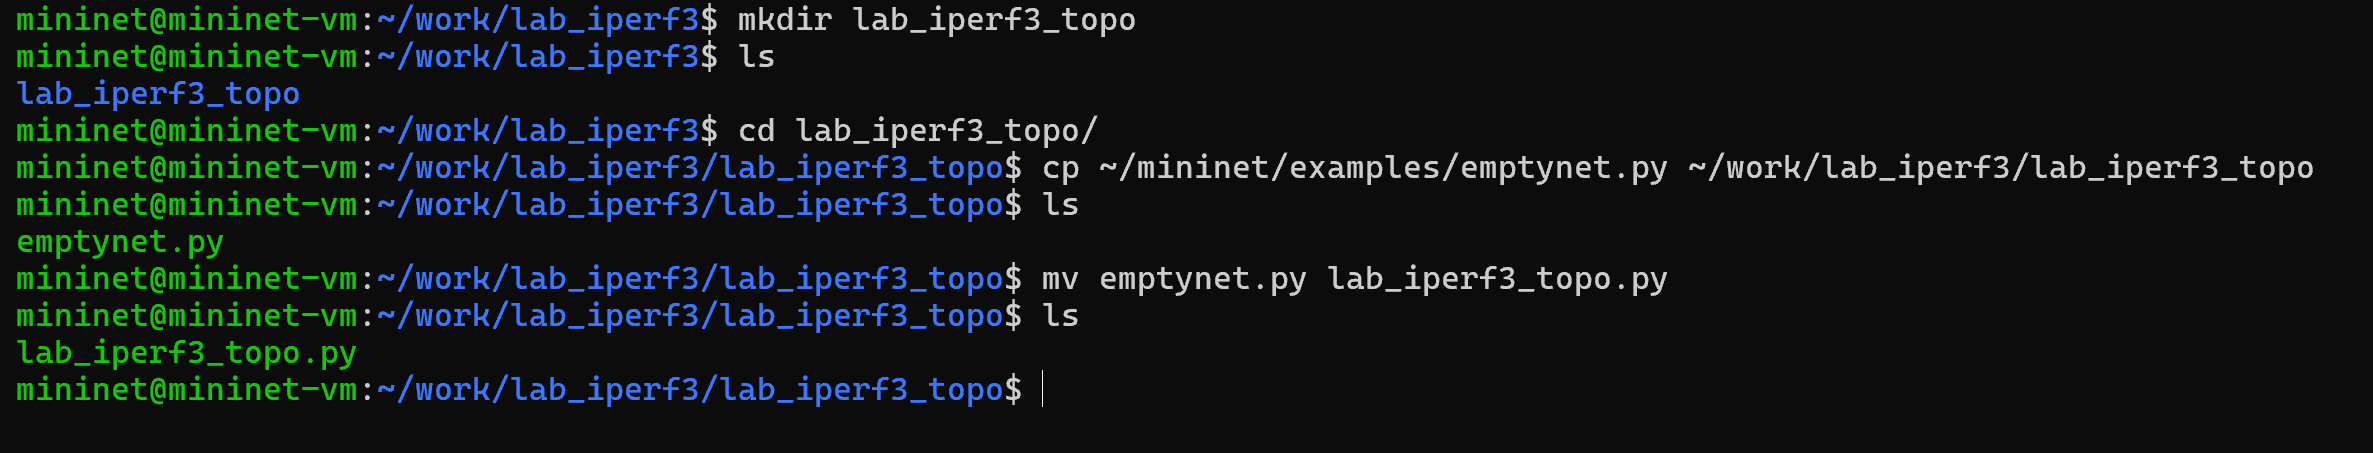
\includegraphics[width=0.7\linewidth,height=\textheight,keepaspectratio]{image/1.png}

}

\caption{\label{fig-001}Копирование файла emptynet.py}

\end{figure}%

Основные элементы:

\begin{itemize}
\tightlist
\item
  addSwitch(): добавляет коммутатор в топологию и возвращает имя
  коммутатора;
\item
  ddHost(): добавляет хост в топологию и возвращает имя хоста;
\item
  addLink(): добавляет двунаправленную ссылку в топологию (и возвращает
  ключ ссылки; ссылки в Mininet являются двунаправленными, если не
  указано иное);
\item
  Mininet: основной класс для создания и управления сетью;
\item
  start(): запускает сеть;
\item
  pingAll(): проверяет подключение, пытаясь заставить все узлы пинговать
  друг друга;
\item
  stop(): останавливает сеть;
\item
  net.hosts: все хосты в сети;
\item
  dumpNodeConnections(): сбрасывает подключения к/от набора узлов;
\item
  setLogLevel( \enquote*{info} \textbar{} \enquote*{debug} \textbar{}
  \enquote*{output} ): устанавливает уровень вывода Mininet по
  умолчанию; рекомендуется info.
\end{itemize}

Запустим скрипт создания топологии lab\_iperf3\_topo.py и посмотрим ее
основные параметры (рис.~\ref{fig-002}).

\begin{figure}

\centering{

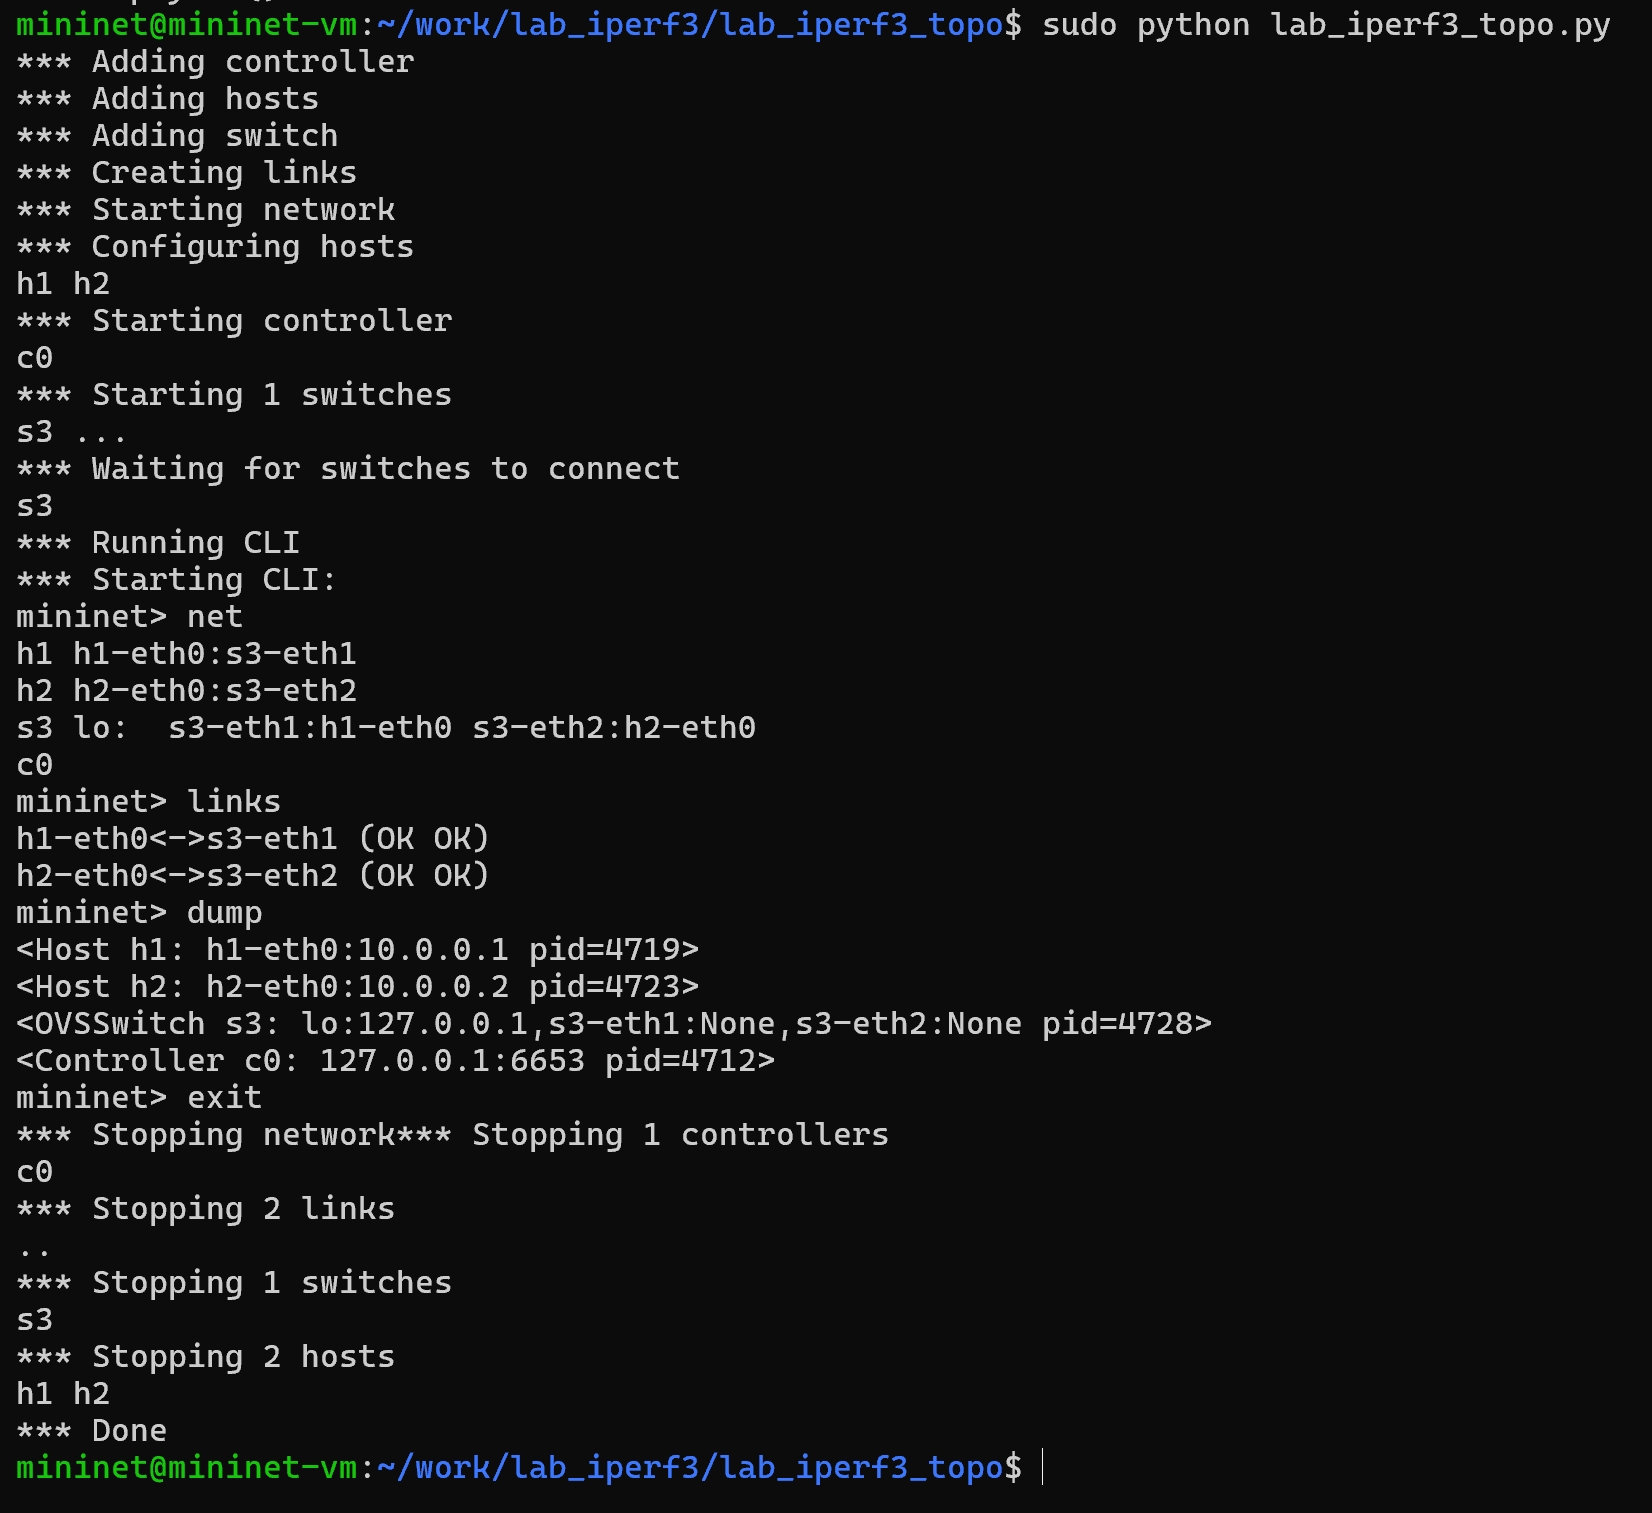
\includegraphics[width=0.7\linewidth,height=\textheight,keepaspectratio]{image/2.png}

}

\caption{\label{fig-002}Создание топологии и ее основные параметры}

\end{figure}%

Внесем в скрипт lab\_iperf3\_topo.py изменение, позволяющее вывести на
экран информацию обоих хостов сети, а именно имя хоста, его IP-адрес,
MAC-адрес (рис.~\ref{fig-003}).

\begin{figure}

\centering{

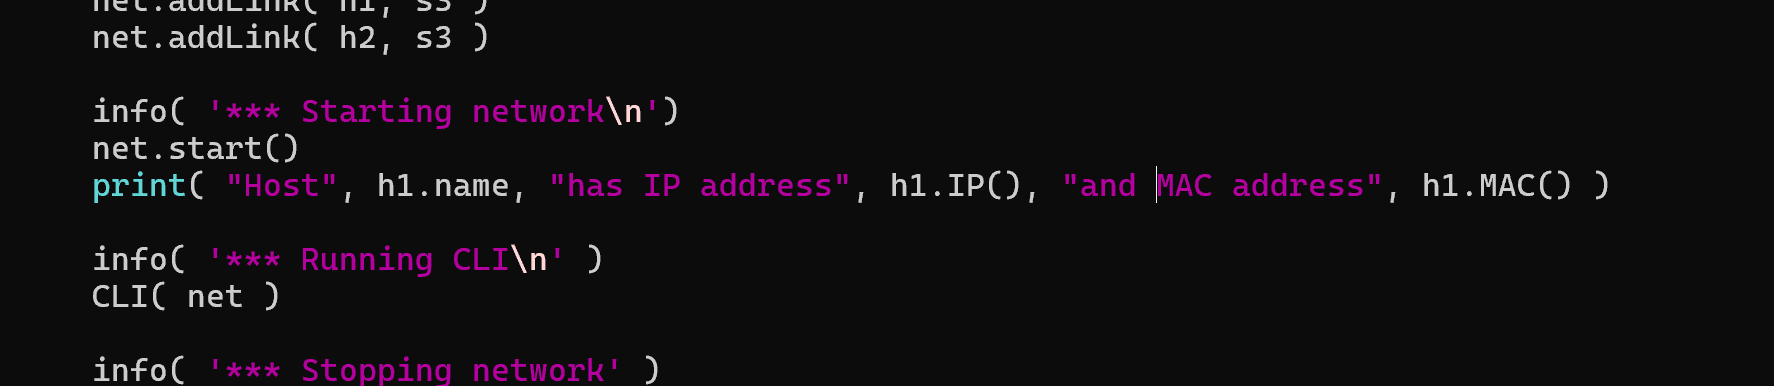
\includegraphics[width=0.7\linewidth,height=\textheight,keepaspectratio]{image/3.png}

}

\caption{\label{fig-003}Изменение скрипта lab\_iperf3\_topo.py}

\end{figure}%

Здесь:

\begin{itemize}
\tightlist
\item
  IP() возвращает IP-адрес хоста или определенного интерфейса;
\item
  MAC() возвращает MAC-адрес хоста или определенного интерфейса.
\end{itemize}

Проверим корректность отработки изменённого скрипта
(рис.~\ref{fig-004}).

\begin{figure}

\centering{

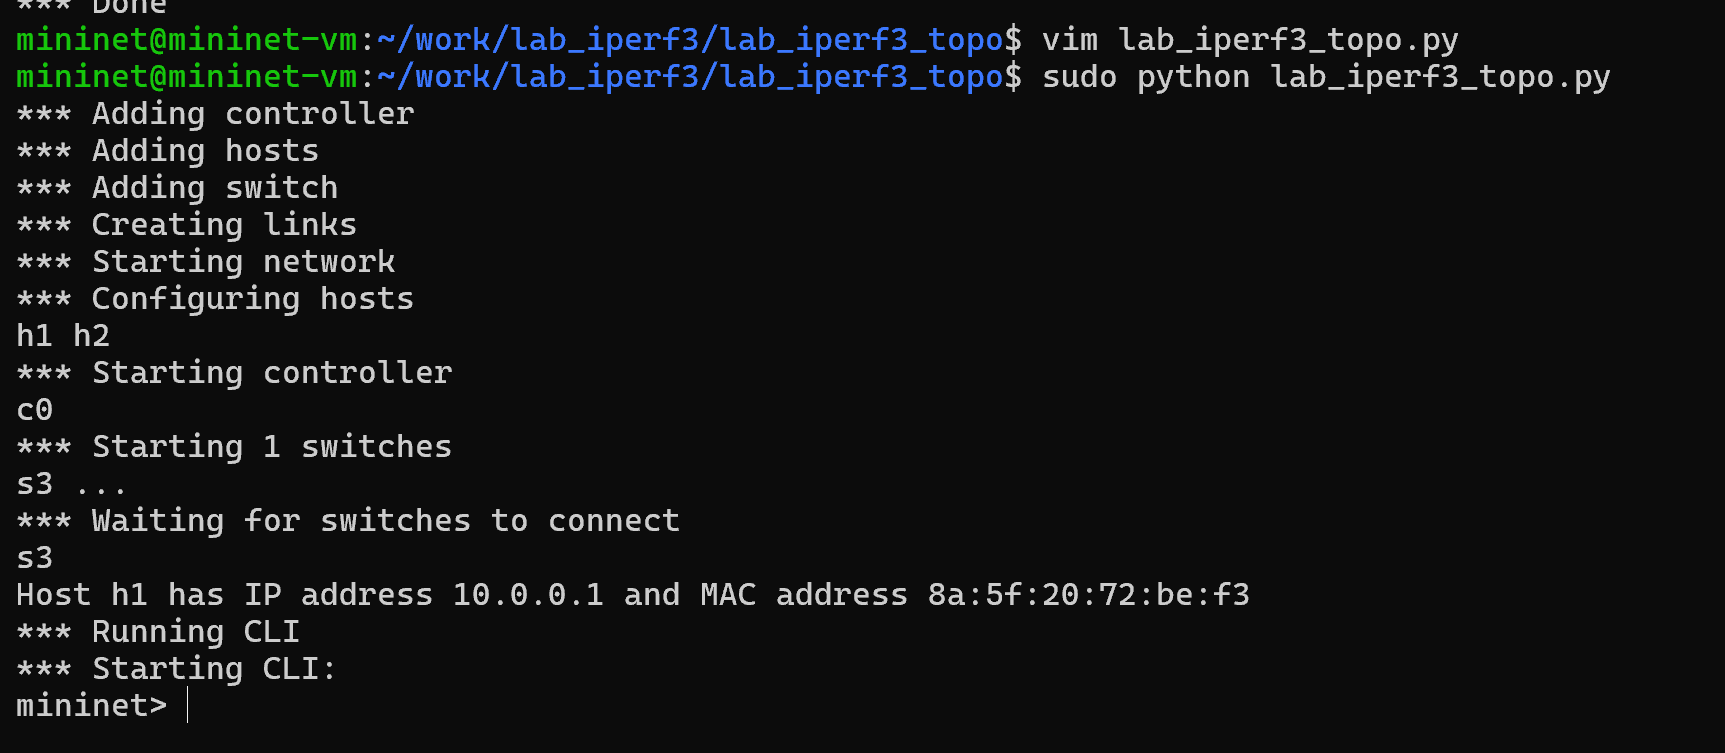
\includegraphics[width=0.7\linewidth,height=\textheight,keepaspectratio]{image/4.png}

}

\caption{\label{fig-004}Проверка работы внесенных изменений}

\end{figure}%

Действительно, нам вывелась информация об IP и mac адресах хостов.
Изменим скрипт lab\_iperf3\_topo.py так, чтобы на экран выводилась
информация об имени, IP-адресе и MAC-адресе обоих хостов сети
(рис.~\ref{fig-005}). Проверим корректность отработки изменённого
скрипта (рис.~\ref{fig-006}).

\begin{figure}

\centering{

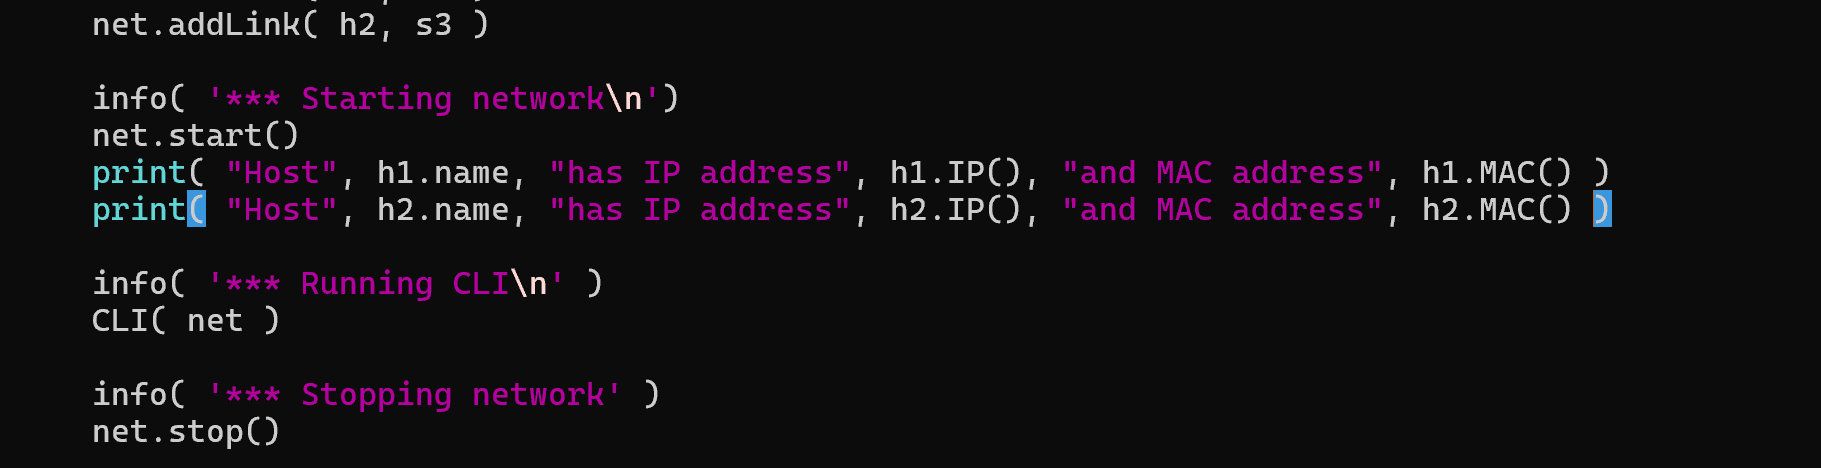
\includegraphics[width=0.7\linewidth,height=\textheight,keepaspectratio]{image/5.png}

}

\caption{\label{fig-005}Изменение скрипта lab\_iperf3\_topo.py}

\end{figure}%

\begin{figure}

\centering{

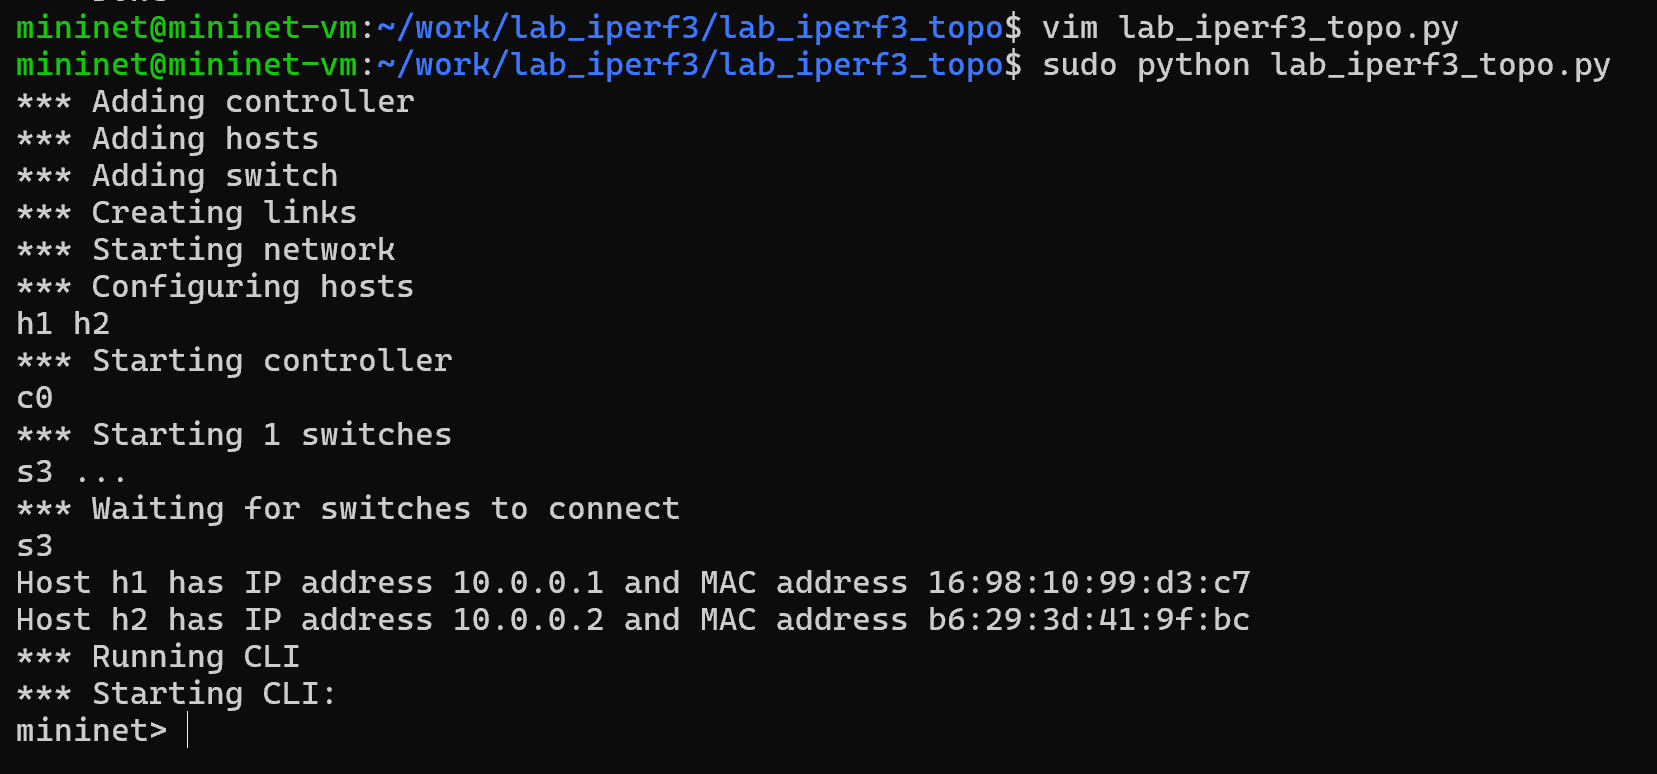
\includegraphics[width=0.7\linewidth,height=\textheight,keepaspectratio]{image/6.png}

}

\caption{\label{fig-006}Проверка работы внесенных изменений}

\end{figure}%

Mininet предоставляет функции ограничения производительности и изоляции
с помощью классов CPULimitedHost и TCLink. Добавим в скрипт настройки
параметров производительности (рис.~\ref{fig-007}).

В скрипте lab\_iperf3\_topo2.py изменим строку описания сети, указав на
использование ограничения производительности и изоляции. Также измении
функцию задания параметров виртуального хоста h1, указав, что ему будет
выделено 50\% от общих ресурсов процессора системы. Аналогичным образом
для хоста h2 зададим долю выделения ресурсов процессора в 45\%. В
скрипте изменим функцию параметров соединения между хостом h1 и
коммутатором s3. А именно добавим двунаправленный канал с
характеристиками пропускной способности, задержки и потерь:

\begin{itemize}
\tightlist
\item
  параметр пропускной способности (bw) выражается числом в Мбит;
\item
  задержка (delay) выражается в виде строки с заданными единицами
  измерения (например, 5ms, 100us, 1s);
\item
  потери (loss) выражаются в процентах (от 0 до 100);
\item
  параметр максимального значения очереди (max\_queue\_size) выражается
  в пакетах;
\item
  параметр use\_htb указывает на использование ограничителя
  интенсивности входящего потока Hierarchical Token Bucket (HTB)
\end{itemize}

\begin{figure}

\centering{

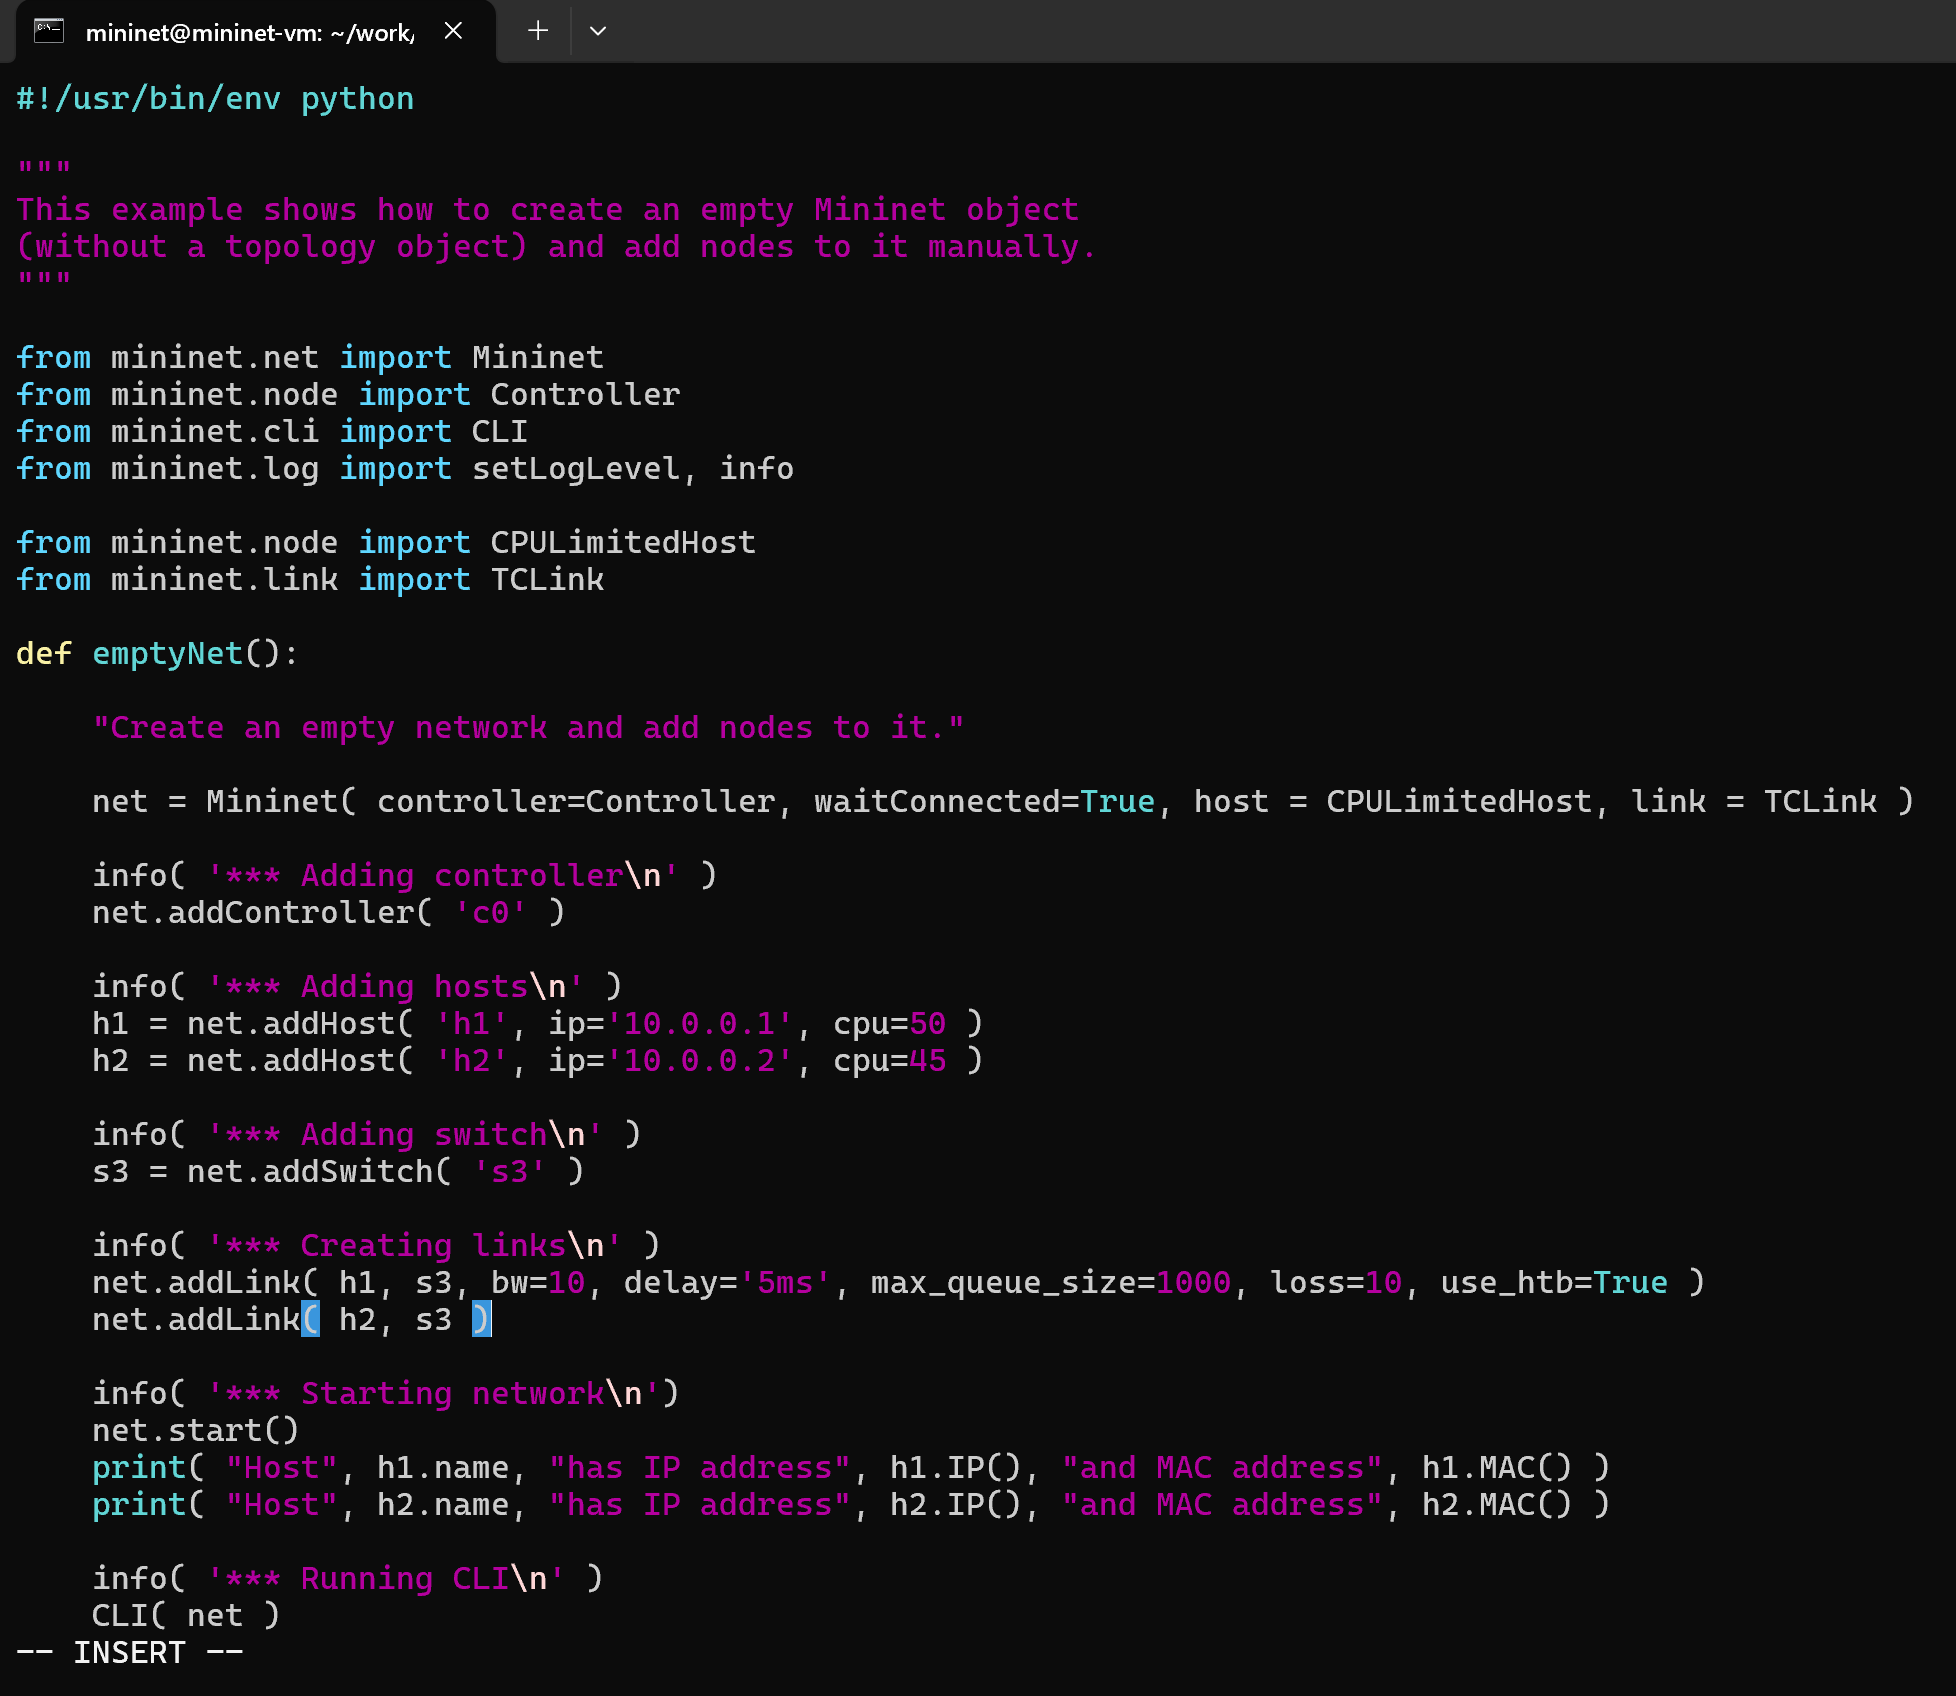
\includegraphics[width=0.7\linewidth,height=\textheight,keepaspectratio]{image/7.png}

}

\caption{\label{fig-007}Настройка параметров производительности}

\end{figure}%

Запустим на отработку сначала скрипт lab\_iperf3\_topo2.py, затем
lab\_iperf3\_topo.py и сравним результат (рис.~\ref{fig-008}). Увидим,
что в первом случае у нас создалась сеть с настроенными параметрами, а
во втором случае дефолтная сеть без этих параметров.

\begin{figure}

\centering{

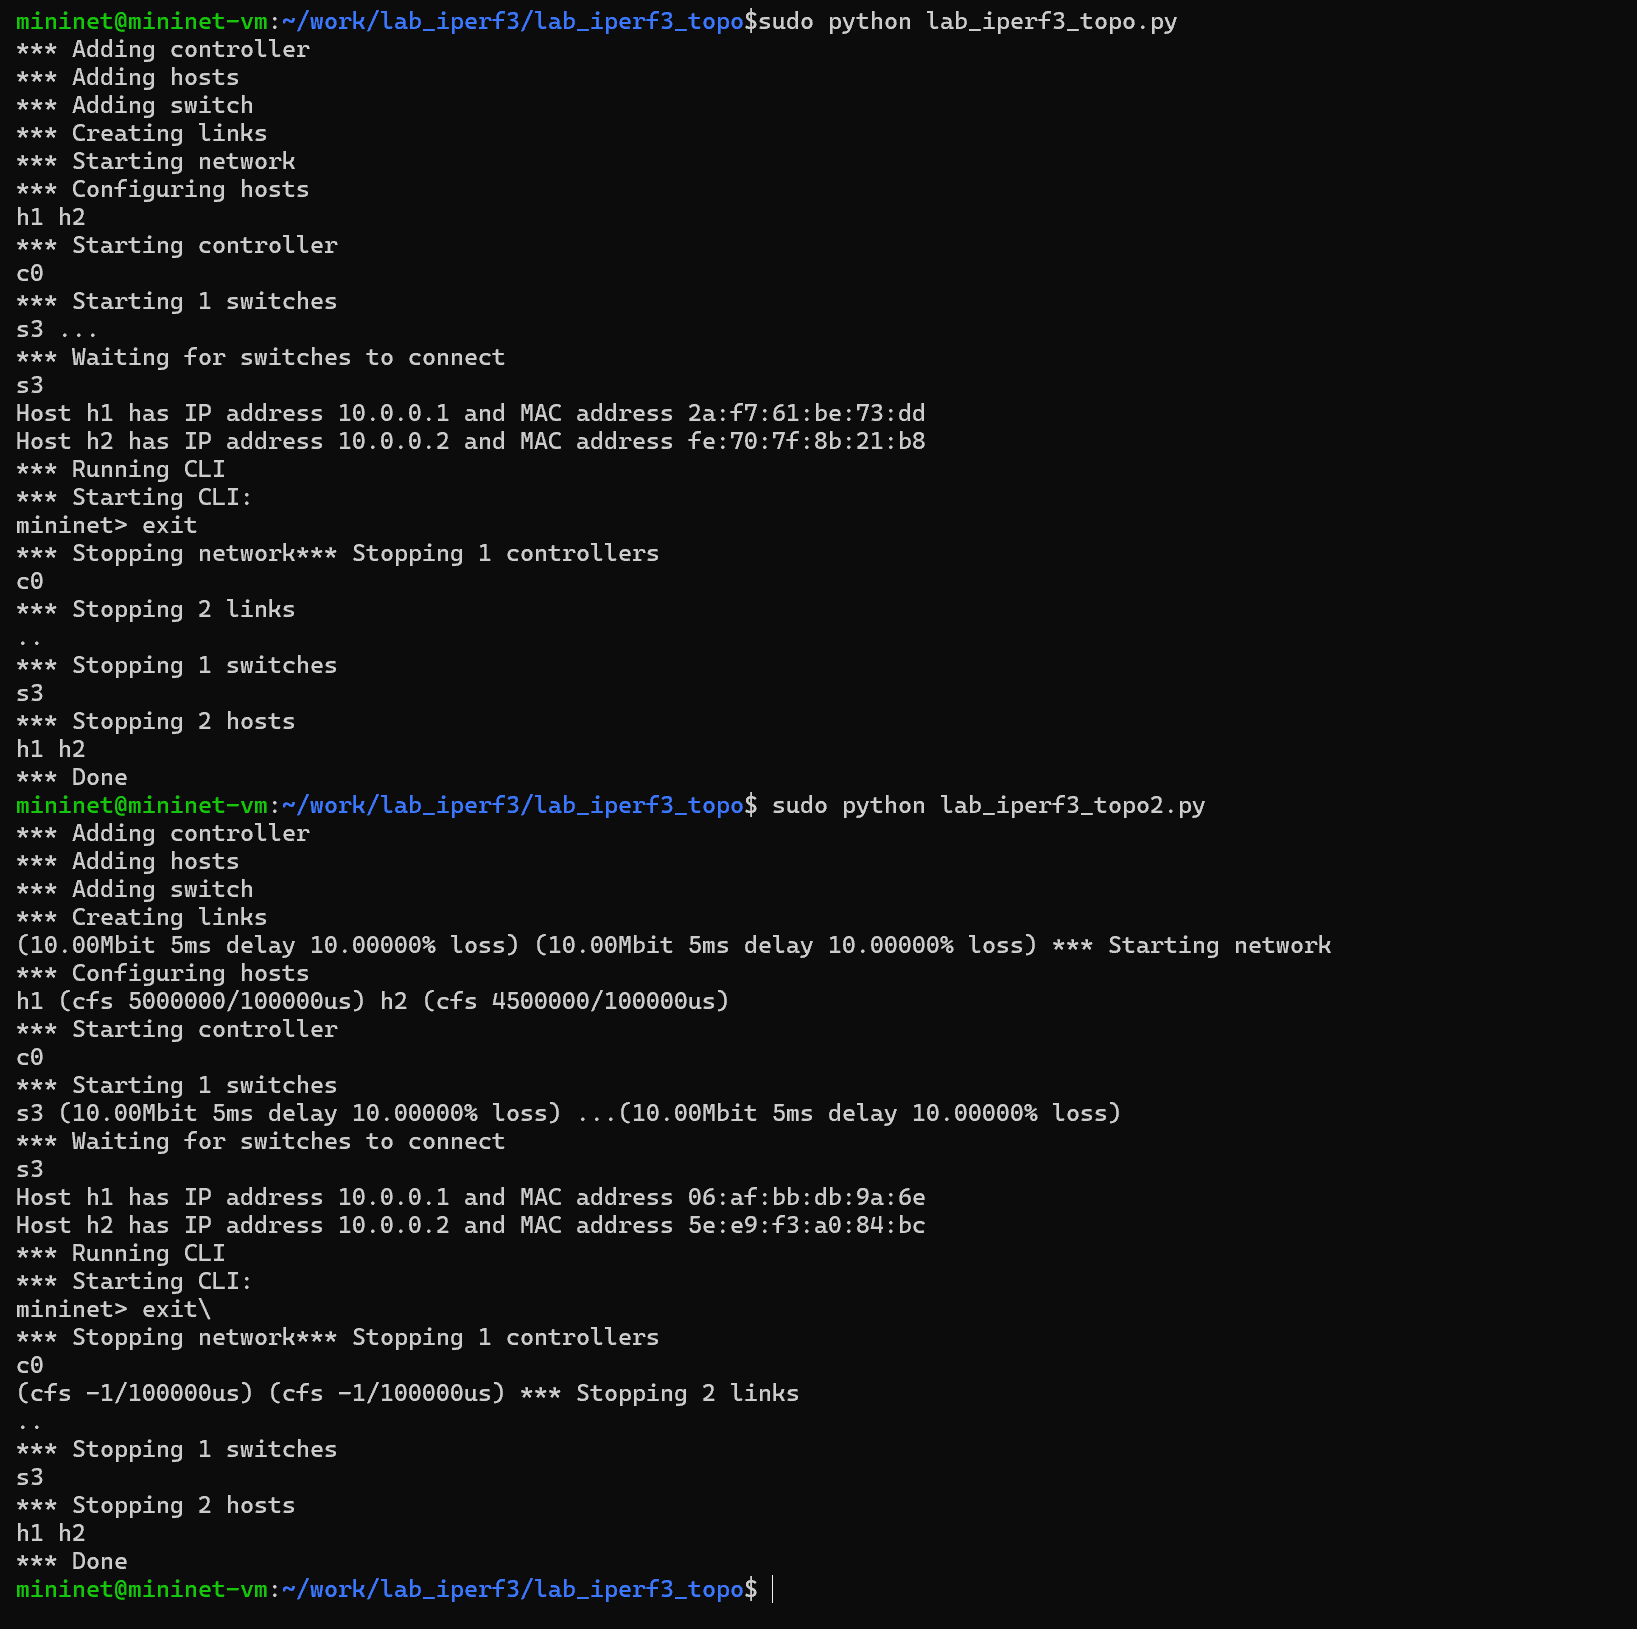
\includegraphics[width=0.7\linewidth,height=\textheight,keepaspectratio]{image/8.png}

}

\caption{\label{fig-008}Запуск скрипта с настройкой параметров
производительности и без нее}

\end{figure}%

Построим графики по проводимому эксперименту.

Сделаем копию скрипта lab\_iperf3\_topo2.py и поместим его в подкаталог
iperf. Изменим код в скрипте lab\_iperf3.py так, чтобы
(рис.~\ref{fig-009}):

\begin{itemize}
\tightlist
\item
  на хостах не было ограничения по использованию ресурсов процессора;
\item
  каналы между хостами и коммутатором были по 100 Мбит/с с задержкой 75
  мс, без потерь, без использования ограничителей пропускной способности
  и максимального размера очереди.
\item
  После функции старта сети опишем запуск на хосте h2 сервера iPerf3, а
  на хосте h1 запуск с задержкой в 10 секунд клиента iPerf3 с экспортом
  результатов в JSON-файл, закомментируем строки, отвечающие за запуск
  CLI-интерфейса:
\end{itemize}

\begin{figure}

\centering{

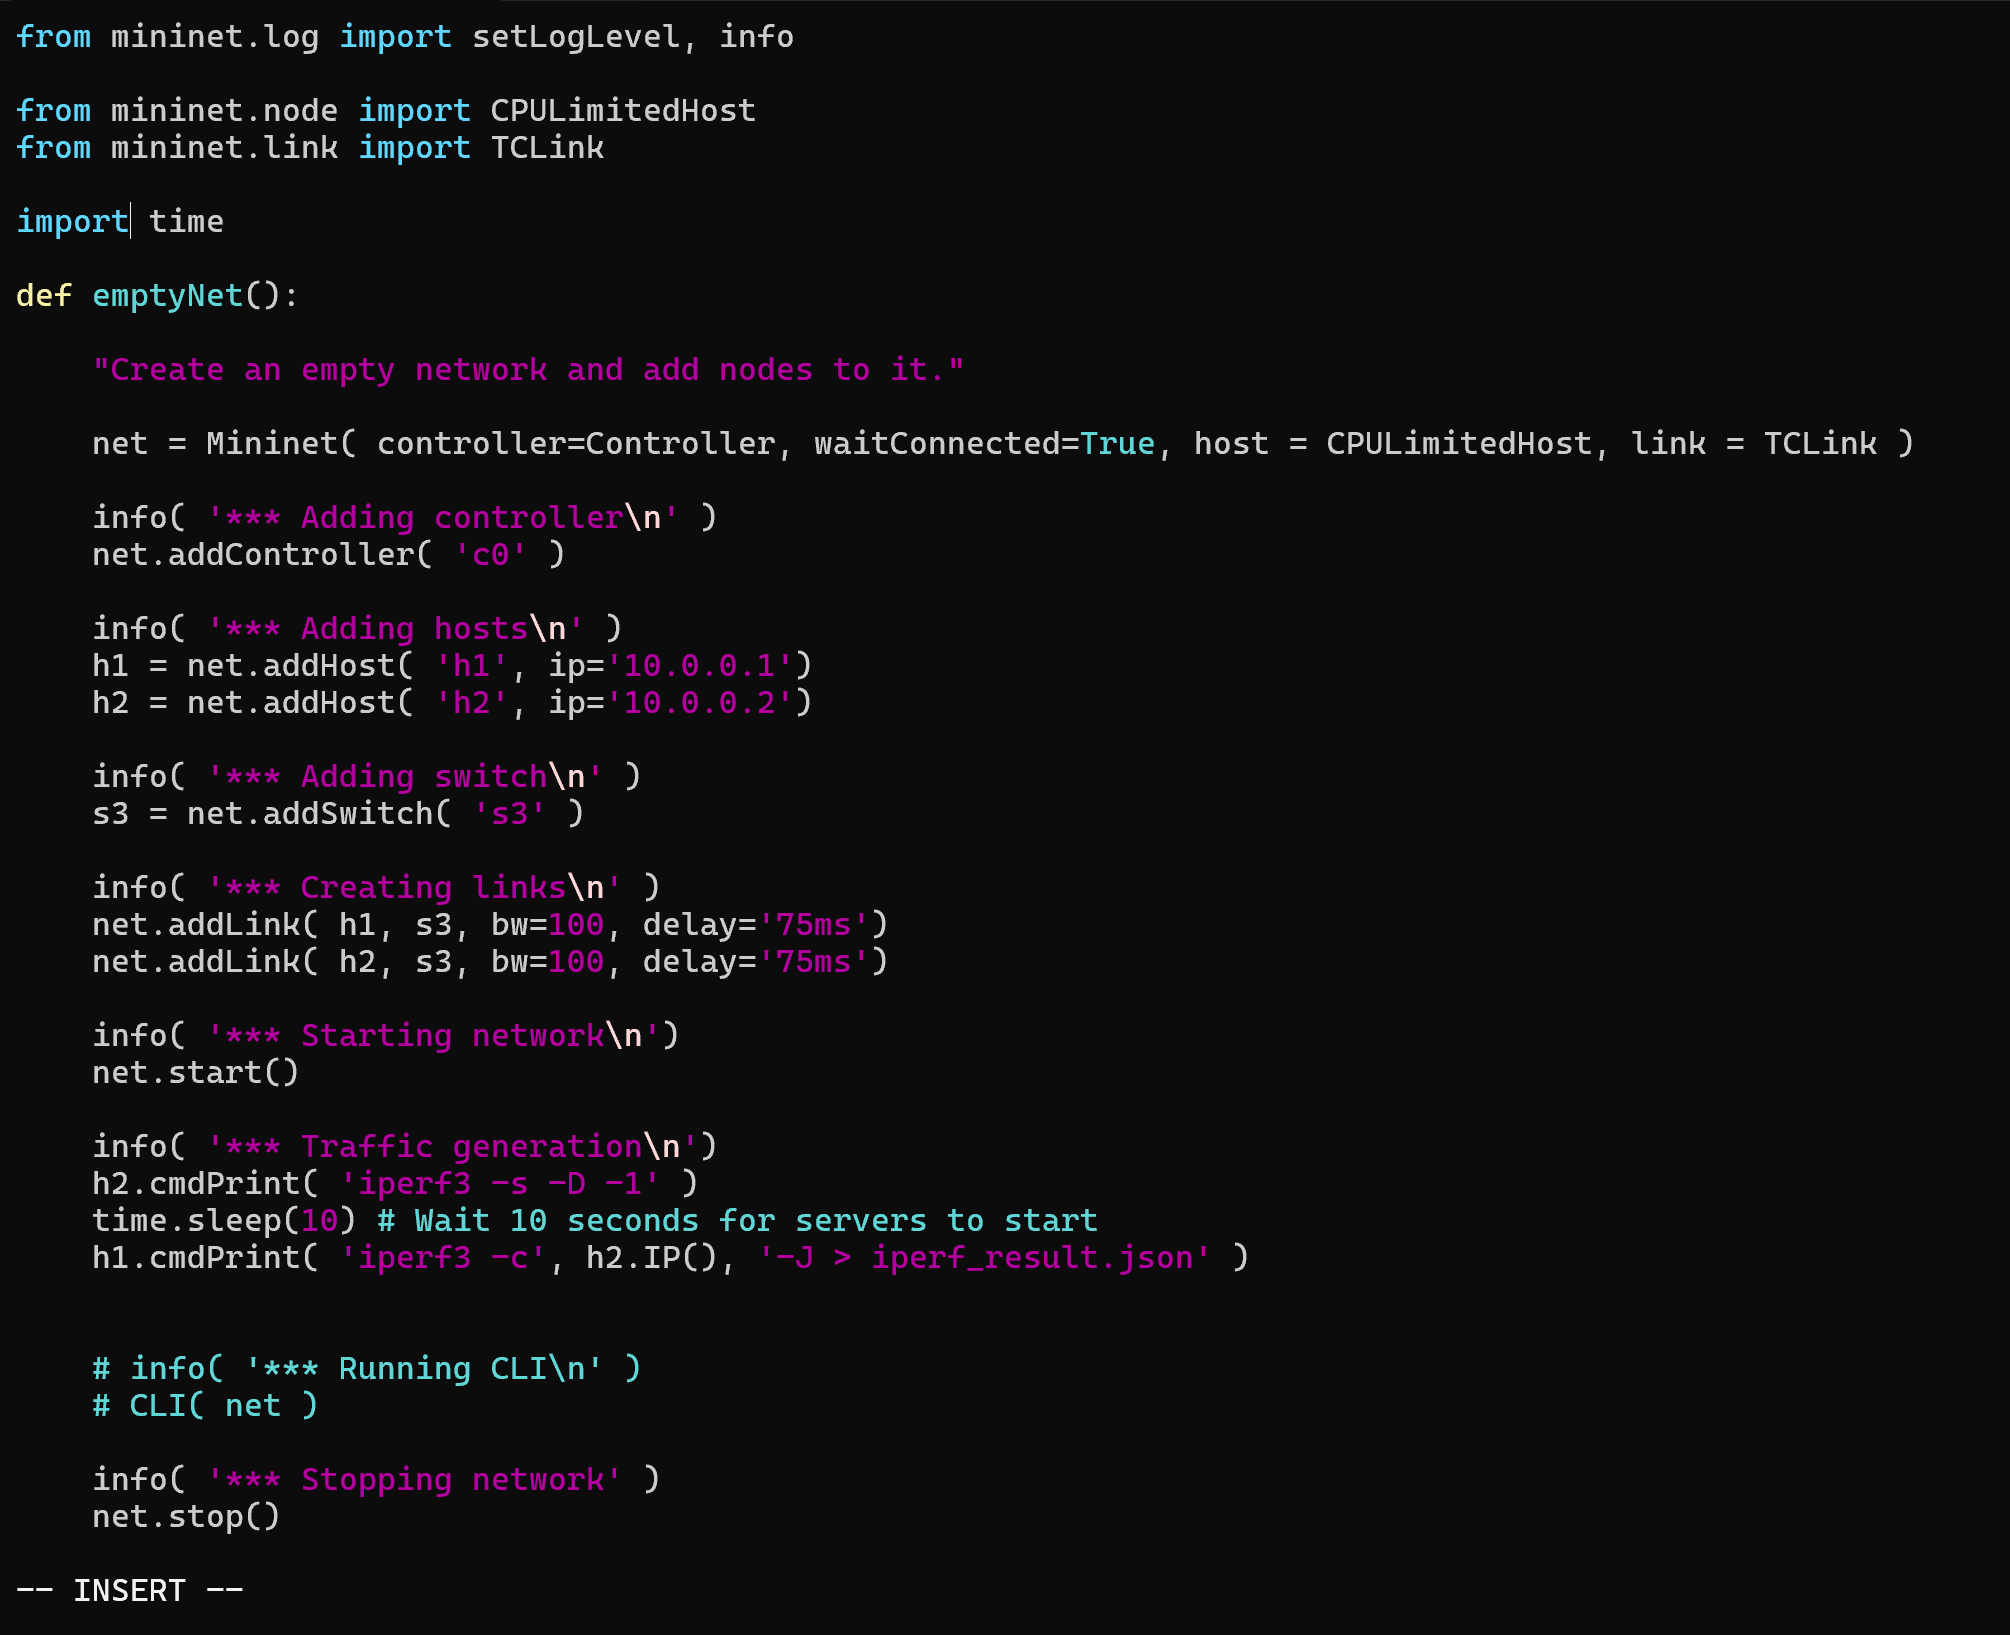
\includegraphics[width=0.7\linewidth,height=\textheight,keepaspectratio]{image/9.png}

}

\caption{\label{fig-009}Изменения кода в скрипте lab\_iperf3.py}

\end{figure}%

Запустим на отработку скрипт lab\_iperf3.py (рис.~\ref{fig-010}).

\begin{figure}

\centering{

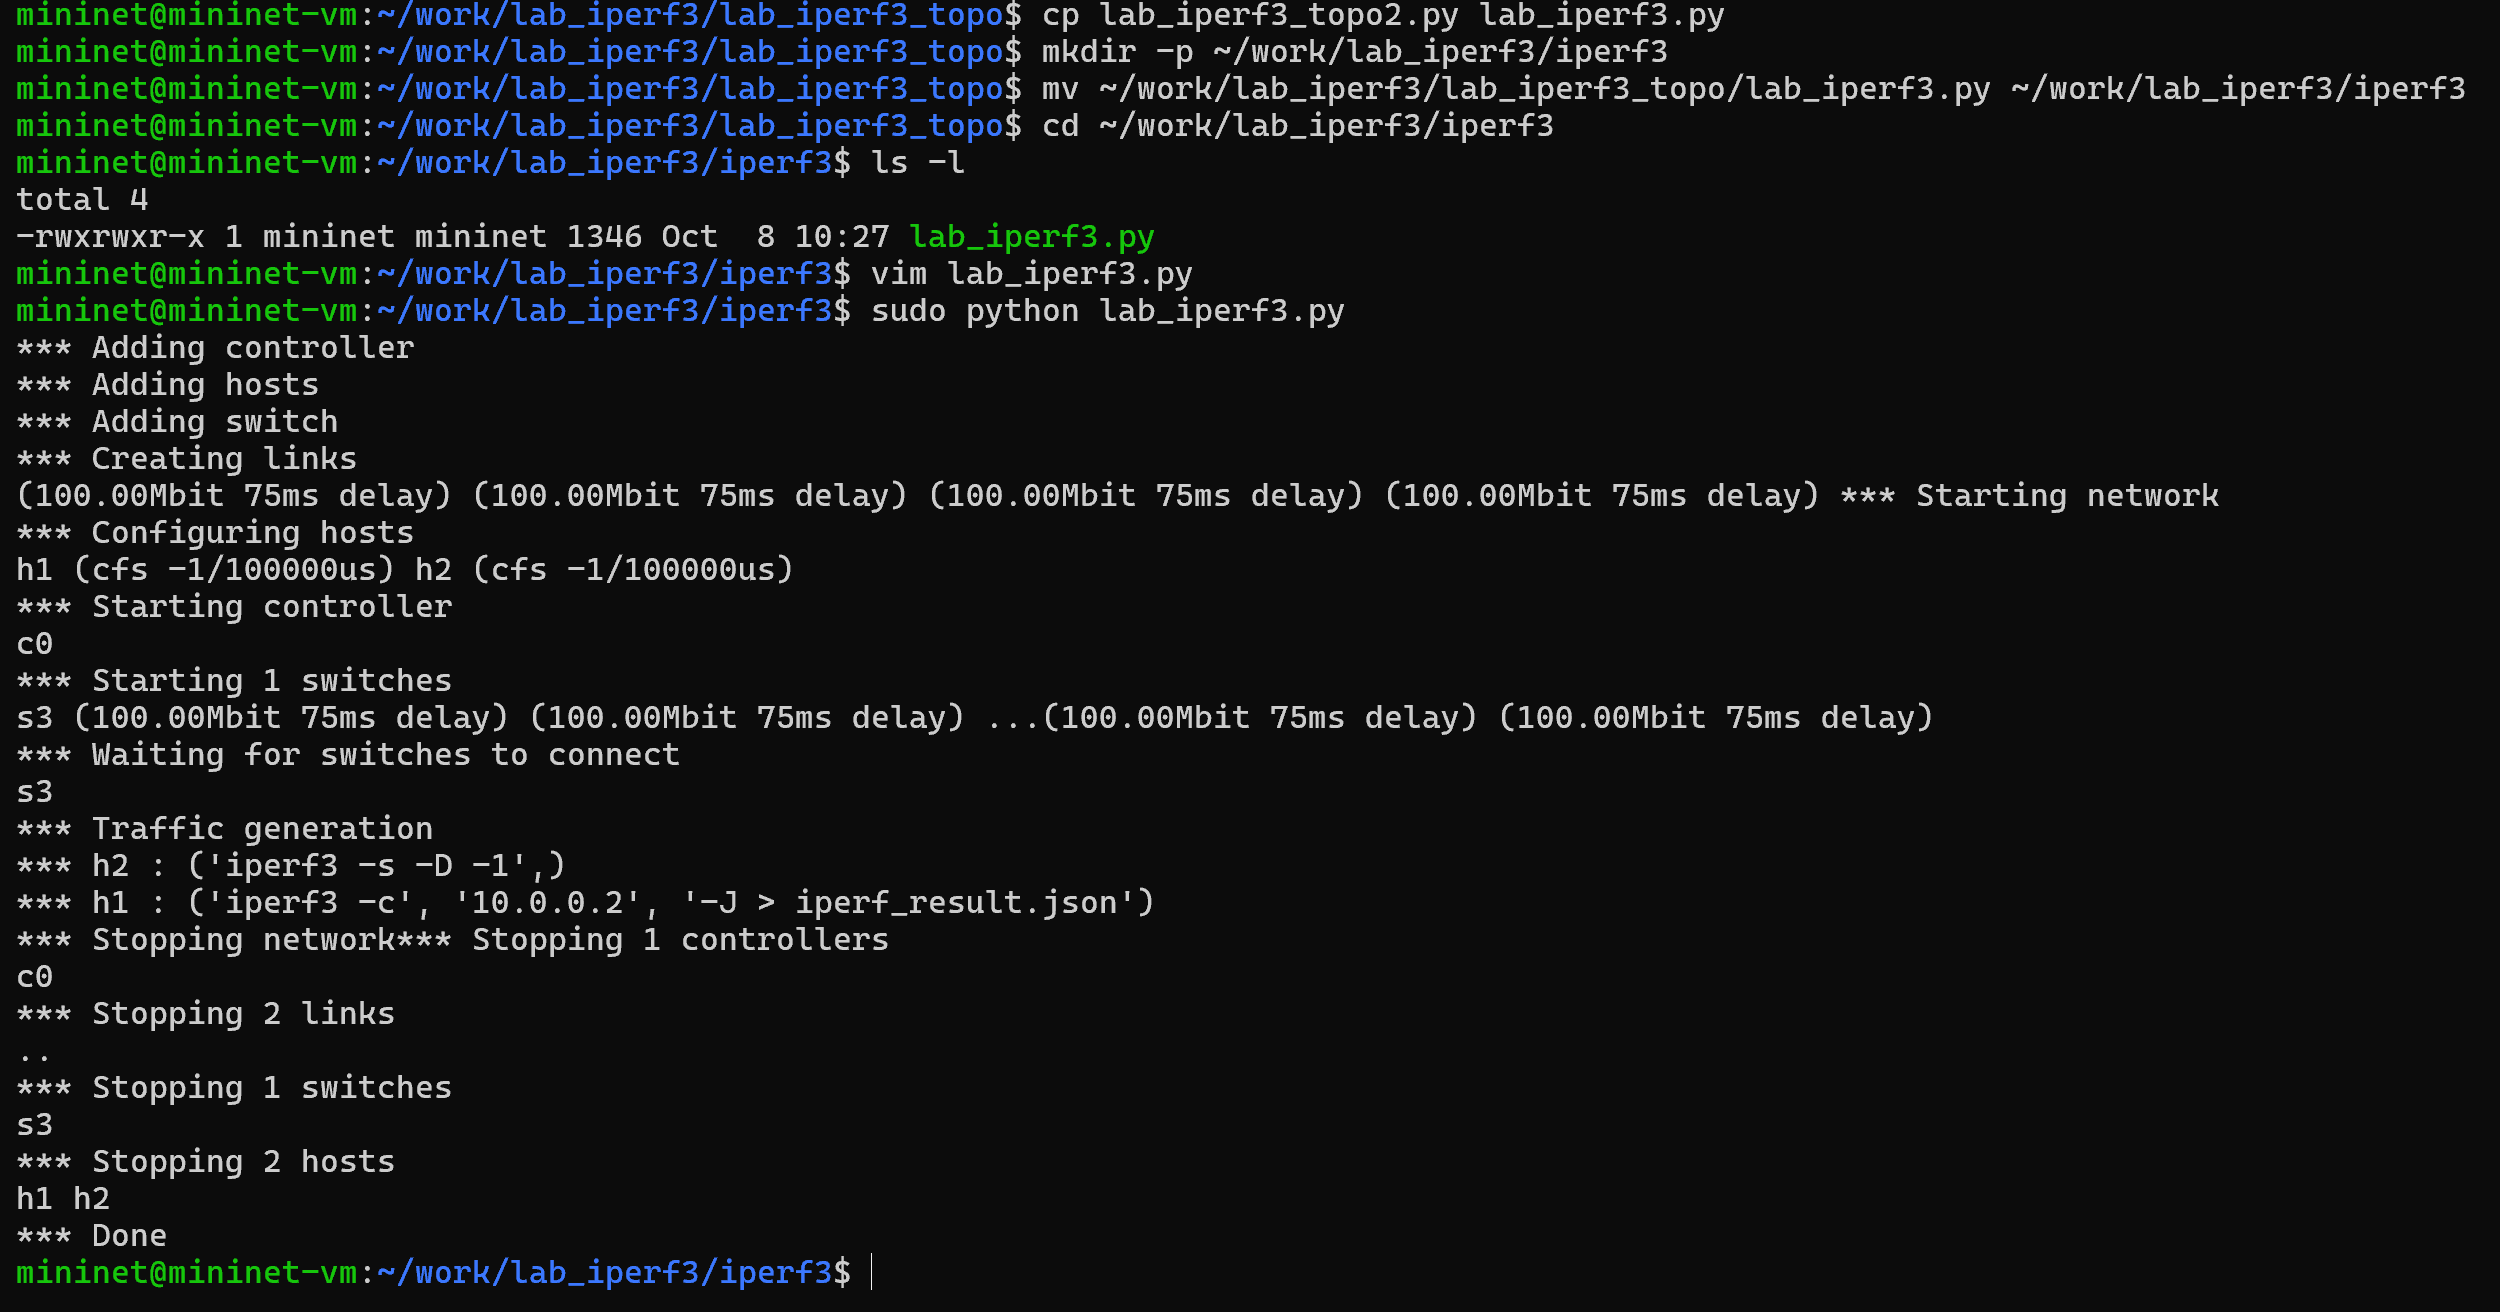
\includegraphics[width=0.7\linewidth,height=\textheight,keepaspectratio]{image/10.png}

}

\caption{\label{fig-010}Запуск скрипта lab\_iperf3.py}

\end{figure}%

Построим графики из получившегося JSON-файла. Создадим Makefile для
проведения всего эксперимента. В Makefile пропишем запуск скрипта
эксперимента, построение графиков и очистку каталога от результатов
(рис.~\ref{fig-011}).

\begin{figure}

\centering{

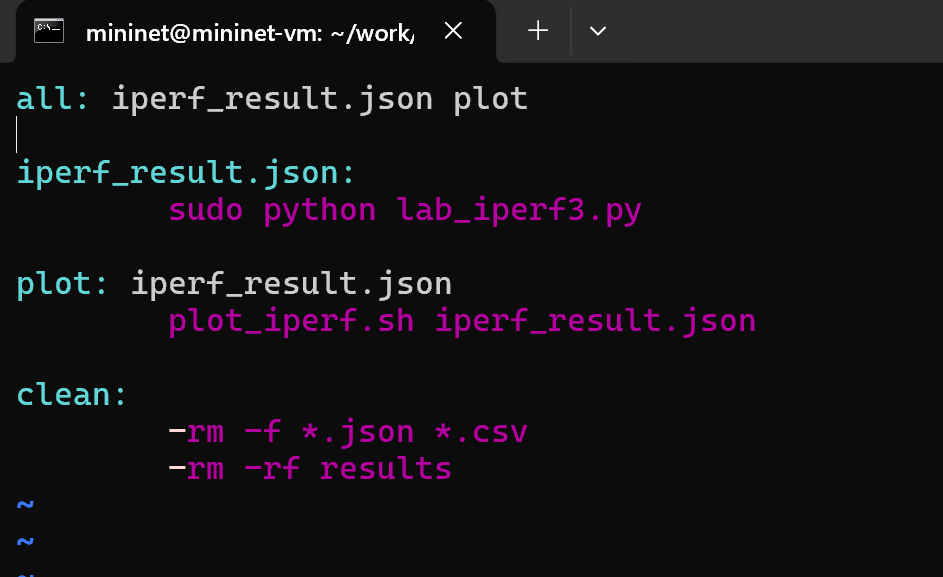
\includegraphics[width=0.7\linewidth,height=\textheight,keepaspectratio]{image/11.png}

}

\caption{\label{fig-011}Создание Makefile}

\end{figure}%

Проверьте корректность отработки Makefile (рис.~\ref{fig-012}).

\begin{figure}

\centering{

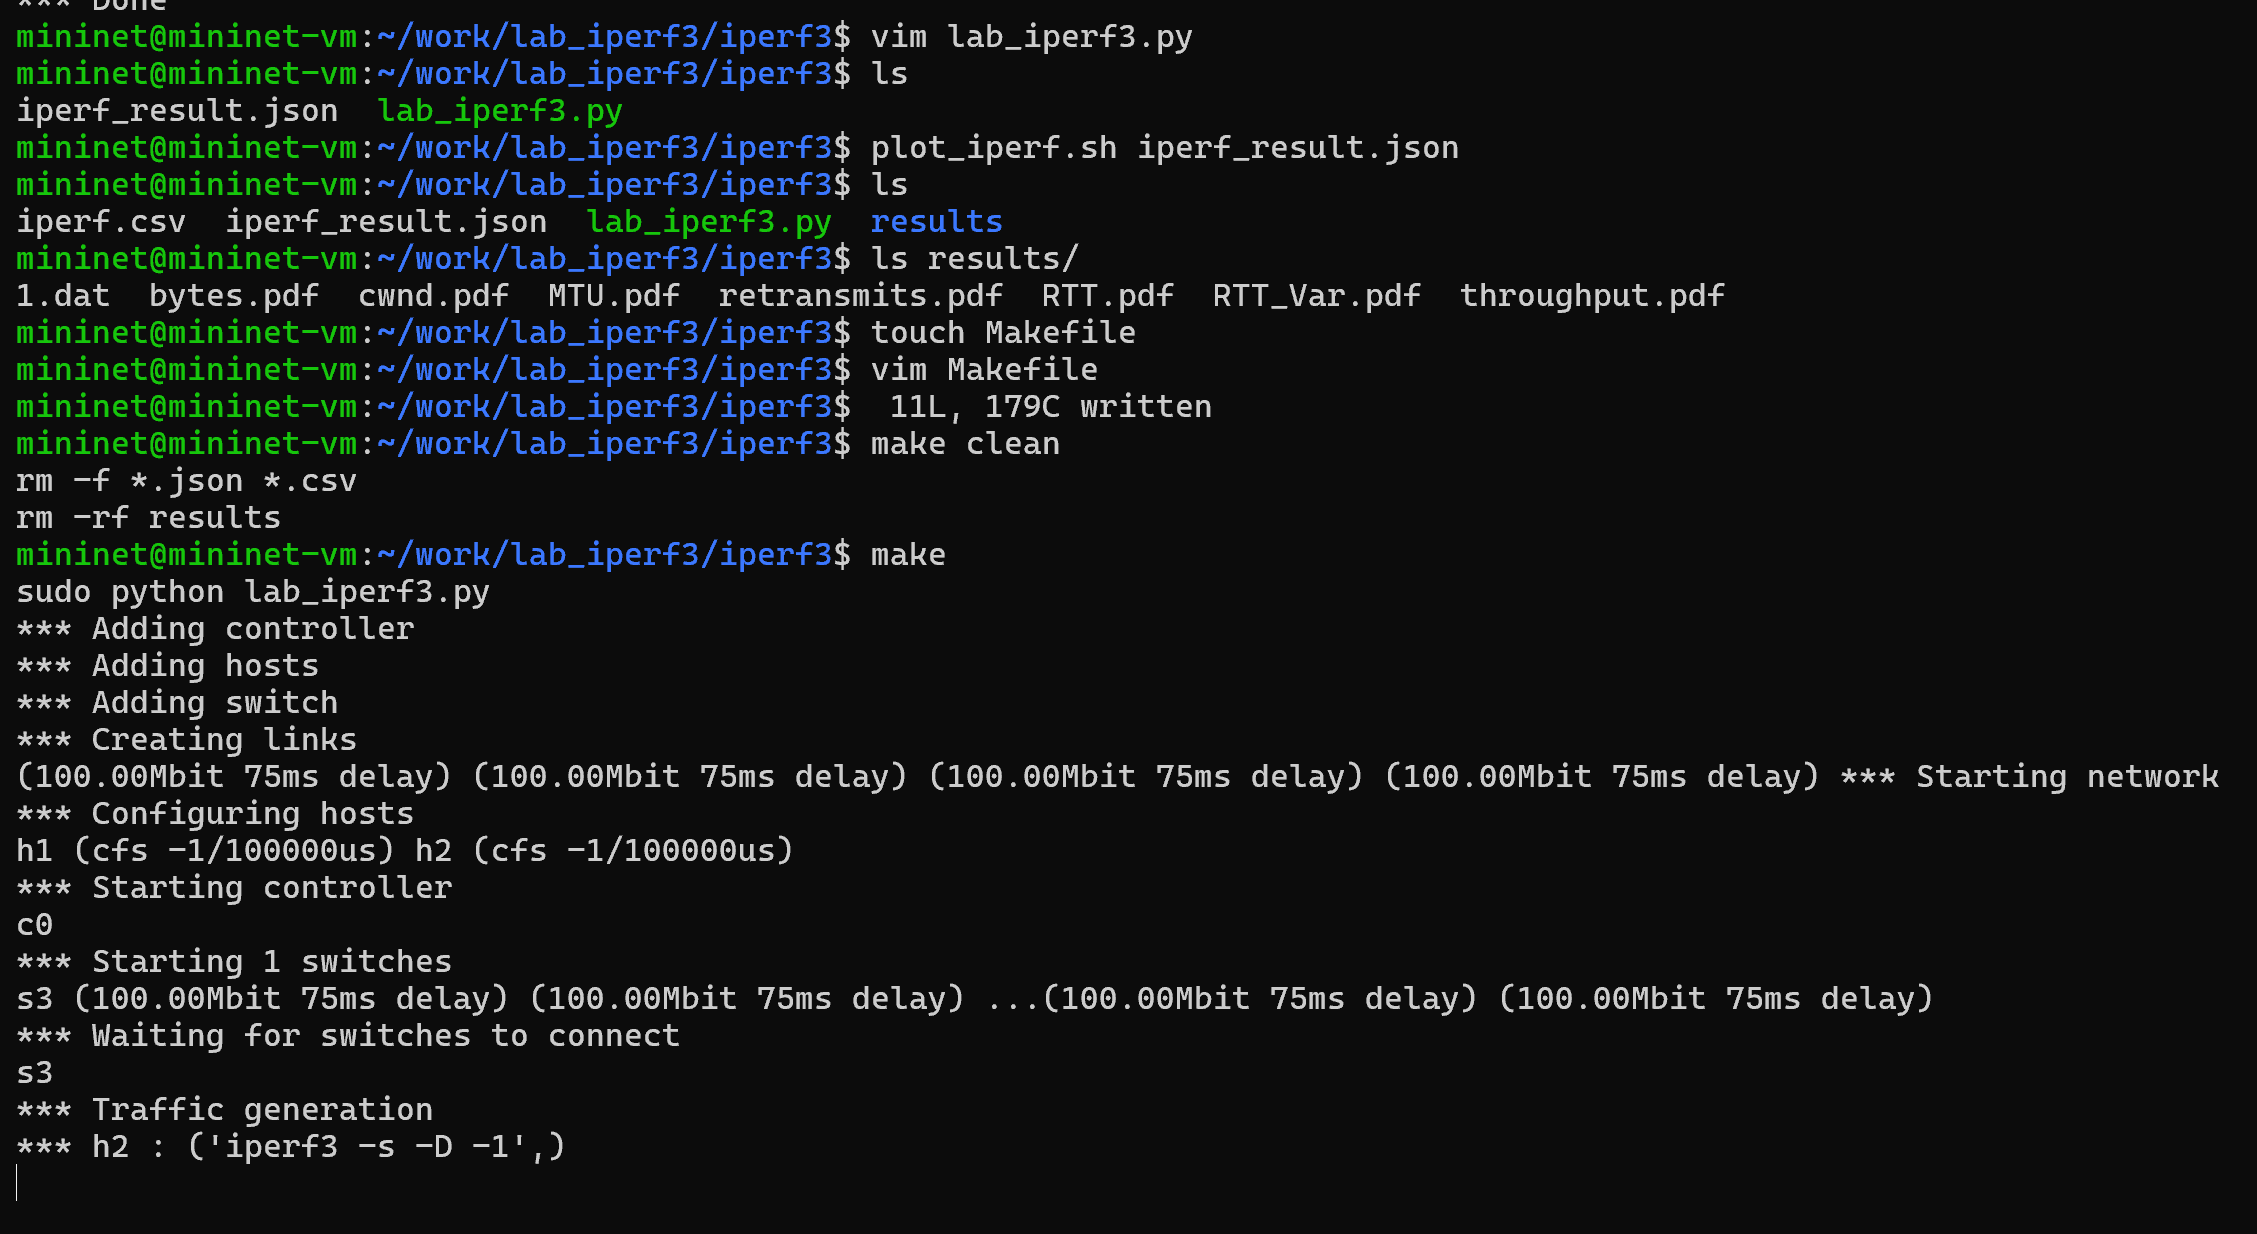
\includegraphics[width=0.7\linewidth,height=\textheight,keepaspectratio]{image/12.png}

}

\caption{\label{fig-012}Проверка работы Makefile}

\end{figure}%

\chapter{Выводы}\label{ux432ux44bux432ux43eux434ux44b}

В результате выполнения данной лабораторной работы я познакомилась с
инструментом для измерения пропускной способности сети в режиме
реального времени --- iPerf3, а также получила навыки проведения
воспроизводимого эксперимента по измерению пропускной способности
моделируемой сети в среде Mininet.

\chapter*{Список
литературы}\label{ux441ux43fux438ux441ux43eux43a-ux43bux438ux442ux435ux440ux430ux442ux443ux440ux44b}
\addcontentsline{toc}{chapter}{Список литературы}

\printbibliography[heading=none]





\end{document}
